\documentclass[journal,12pt,twocolumn]{IEEEtran}
%
\usepackage{setspace}
\usepackage{gensymb}
\usepackage{siunitx}
\usepackage{tkz-euclide} 
\usepackage{textcomp}
\usepackage{standalone}
\usetikzlibrary{calc}
\newcommand\hmmax{0}
\newcommand\bmmax{0}

%\doublespacing
\singlespacing

%\usepackage{graphicx}
%\usepackage{amssymb}
%\usepackage{relsize}
\usepackage[cmex10]{amsmath}
%\usepackage{amsthm}
%\interdisplaylinepenalty=2500
%\savesymbol{iint}
%\usepackage{txfonts}
%\restoresymbol{TXF}{iint}
%\usepackage{wasysym}
\usepackage{amsthm}
%\usepackage{iithtlc}
\usepackage{mathrsfs}
\usepackage{txfonts}
\usepackage{stfloats}
\usepackage{bm}
\usepackage{cite}
\usepackage{cases}
\usepackage{subfig}
%\usepackage{xtab}
\usepackage{longtable}
\usepackage{multirow}
%\usepackage{algorithm}
%\usepackage{algpseudocode}
\usepackage{enumitem}
\usepackage{mathtools}
\usepackage{steinmetz}
\usepackage{tikz}
\usepackage{circuitikz}
\usepackage{verbatim}
\usepackage{tfrupee}
\usepackage[breaklinks=true]{hyperref}
%\usepackage{stmaryrd}
\usepackage{tkz-euclide} % loads  TikZ and tkz-base
%\usetkzobj{all}
\usetikzlibrary{calc,math}
\usepackage{listings}
    \usepackage{color}                                            %%
    \usepackage{array}                                            %%
    \usepackage{longtable}                                        %%
    \usepackage{calc}                                             %%
    \usepackage{multirow}                                         %%
    \usepackage{hhline}                                           %%
    \usepackage{ifthen}                                           %%
  %optionally (for landscape tables embedded in another document): %%
    \usepackage{lscape}     
\usepackage{multicol}
\usepackage{chngcntr}
\usepackage{amsmath}
\usepackage{cleveref}
\usepackage{amsmath}
%\usepackage{enumerate}

%\usepackage{wasysym}
%\newcounter{MYtempeqncnt}
\DeclareMathOperator*{\Res}{Res}
%\renewcommand{\baselinestretch}{2}
\renewcommand\thesection{\arabic{section}}
\renewcommand\thesubsection{\thesection.\arabic{subsection}}
\renewcommand\thesubsubsection{\thesubsection.\arabic{subsubsection}}

\renewcommand\thesectiondis{\arabic{section}}
\renewcommand\thesubsectiondis{\thesectiondis.\arabic{subsection}}
\renewcommand\thesubsubsectiondis{\thesubsectiondis.\arabic{subsubsection}}

% correct bad hyphenation here
\hyphenation{op-tical net-works semi-conduc-tor}
\def\inputGnumericTable{}                                 %%

\lstset{
%language=C,
frame=single, 
breaklines=true,
columns=fullflexible
}
%\lstset{
%language=tex,
%frame=single, 
%breaklines=true
%}
\usepackage{graphicx}
\usepackage{pgfplots}

\begin{document}


\newtheorem{theorem}{Theorem}[section]
\newtheorem{problem}{Problem}
\newtheorem{proposition}{Proposition}[section]
\newtheorem{lemma}{Lemma}[section]
\newtheorem{corollary}[theorem]{Corollary}
\newtheorem{example}{Example}[section]
\newtheorem{definition}[problem]{Definition}
%\newtheorem{thm}{Theorem}[section] 
%\newtheorem{defn}[thm]{Definition}
%\newtheorem{algorithm}{Algorithm}[section]
%\newtheorem{cor}{Corollary}
\newcommand{\BEQA}{\begin{eqnarray}}
\newcommand{\EEQA}{\end{eqnarray}}
\newcommand{\define}{\stackrel{\triangle}{=}}
\bibliographystyle{IEEEtran}
%\bibliographystyle{ieeetr}
\providecommand{\mbf}{\mathbf}
\providecommand{\abs}[1]{\ensuremath{\left\vert#1\right\vert}}
\providecommand{\norm}[1]{\ensuremath{\left\lVert#1\right\rVert}}
\providecommand{\mean}[1]{\ensuremath{E\left[ #1 \right]}}
\providecommand{\pr}[1]{\ensuremath{\Pr\left(#1\right)}}
\providecommand{\qfunc}[1]{\ensuremath{Q\left(#1\right)}}
\providecommand{\sbrak}[1]{\ensuremath{{}\left[#1\right]}}
\providecommand{\lsbrak}[1]{\ensuremath{{}\left[#1\right.}}
\providecommand{\rsbrak}[1]{\ensuremath{{}\left.#1\right]}}
\providecommand{\brak}[1]{\ensuremath{\left(#1\right)}}
\providecommand{\lbrak}[1]{\ensuremath{\left(#1\right.}}
\providecommand{\rbrak}[1]{\ensuremath{\left.#1\right)}}
\providecommand{\cbrak}[1]{\ensuremath{\left\{#1\right\}}}
\providecommand{\lcbrak}[1]{\ensuremath{\left\{#1\right.}}
\providecommand{\rcbrak}[1]{\ensuremath{\left.#1\right\}}}
\theoremstyle{remark}
\newtheorem{rem}{Remark}
\newcommand{\sgn}{\mathop{\mathrm{sgn}}}
\providecommand{\res}[1]{\Res\displaylimits_{#1}} 
%\providecommand{\norm}[1]{\lVert#1\rVert}
\providecommand{\mtx}[1]{\mathbf{#1}}
\providecommand{\fourier}{\overset{\mathcal{F}}{ \rightleftharpoons}}
%\providecommand{\hilbert}{\overset{\mathcal{H}}{ \rightleftharpoons}}
\providecommand{\system}{\overset{\mathcal{H}}{ \longleftrightarrow}}
	%\newcommand{\solution}[2]{\textbf{Solution:}{#1}}
\newcommand{\solution}{\noindent \textbf{Solution: }}
\newcommand{\cosec}{\,\text{cosec}\,}
\providecommand{\dec}[2]{\ensuremath{\overset{#1}{\underset{#2}{\gtrless}}}}
\newcommand{\myvec}[1]{\ensuremath{\begin{pmatrix}#1\end{pmatrix}}}
\newcommand{\mydet}[1]{\ensuremath{\begin{vmatrix}#1\end{vmatrix}}}
%\numberwithin{equation}{section}
\numberwithin{equation}{subsection}
%\numberwithin{problem}{section}
%\numberwithin{definition}{section}
\makeatletter
\@addtoreset{figure}{problem}
\makeatother
\let\StandardTheFigure\thefigure
\let\vec\mathbf
%\renewcommand{\thefigure}{\theproblem.\arabic{figure}}
\renewcommand{\thefigure}{\theproblem}
%\setlist[enumerate,1]{before=\renewcommand\theequation{\theenumi.\arabic{equation}}
%\counterwithin{equation}{enumi}
%\renewcommand{\theequation}{\arabic{subsection}.\arabic{equation}}
\def\putbox#1#2#3{\makebox[0in][l]{\makebox[#1][l]{}\raisebox{\baselineskip}[0in][0in]{\raisebox{#2}[0in][0in]{#3}}}}
     \def\rightbox#1{\makebox[0in][r]{#1}}
     \def\centbox#1{\makebox[0in]{#1}}
     \def\topbox#1{\raisebox{-\baselineskip}[0in][0in]{#1}}
\vspace{3cm}
\title{Evidence Function}
\maketitle
\newpage
%\tableofcontents
\bigskip
\renewcommand{\thefigure}{\theenumi}
\renewcommand{\thetable}{\theenumi}
\begin{abstract}
This document contains theory involved in curve fitting.
\end{abstract}
\section{\textbf{Objective}}
The objective is to evaluate the evidence function.
\section{Generate Dataset}
Create a sinusoidal function of the form
\begin{align}
    y = A\sin{2\pi x} + n(t) \label{eq:1}
\end{align}
n(t) is the random noise that is included in the training set. This set consists of N samples of input data i.e. x expressed as shown below
\begin{align}
    x = \myvec{x_{1}, x_{2}, .., x_{N}}^{T}
\end{align}
which give the corresponding values of y denoted as
\begin{align}
    y = \myvec{y_{1}, y_{2}, .., y_{N}}^{T}
\end{align}

The corresponding values of y are generated from the Eq \eqref{eq:1}.The first term $A\sin{2\pi x}$ is computed directly and then random noise samples having a normal(Gaussian) distribution are added inorder to get the corresponding values of y.
\begin{lstlisting}
#Generate the sine curve 
def g(X, noise_variance):
    '''Sinusoidal function plus noise'''
    return 0.5 + np.sin(2 * np.pi * X) + noise(X.shape, noise_variance)
\end{lstlisting}

The generated input matrix would look like
\begin{align}
    \vec{F}= \myvec{ 1 & x_{0} & x_{0}^2 & \ldots & x_{0}^{N-1} \\
		1 & x_{1} & x_{1}^2 & \ldots & x_{1}^{N-1} \\
		1 & x_{2} & x_{2}^2 & \ldots & x_{2}^{N-1} \\
		\vdots & & \vdots &  & \vdots  \\
		    1 & \ldots & \ldots & \ldots & x_{N}^{N-1} }\label{eq:12}
\end{align}
\section{Polynomial Curve Fitting}
The goal is to find the best line that fits into the  pattern of the training data shown in the graph.
We shall fit the data using a polynomial function of the form, 
\begin{align}
     y\brak{w,x}= \sum_{j=0}^{M} w_j x^{j}\\
\end{align}
M is the order of the polynomial
The polynomial coefficient are collectively denoted by the vector $\vec{w}$.The proposed vector $\vec{w}$ of the model referring to Eq \eqref{eq:12} is given by 
\begin{align}
    \hat{\vec{w}} = \brak{\vec{F}^T\vec{F}}^{-1}\vec{F}^Ty \label{eq:13}
\end{align}

\section{Evidence Function}
For Bayesian treatment of linear regression, we introduce a prior probability distribution over the model parameters $\vec{w}$.

The corresponding conjugate prior is therefore given by a Gaussian
distribution of the form
\begin{align}
    p(\vec{w}) = N(\vec{w} | \vec{m_{0}},\vec{S_{0}})
\end{align}
having mean $\vec{m_{0}}$ and covariance $\vec{S_{0}}$.

We now compute the posterior distribution, which is proportional to the product of the likelihood function and the prior which takes the form
\begin{align}
    p(\vec{w} | t) = N(\vec{w} | \vec{m_{N}},\vec{S_{N}}) \label{eq : posterior}
\end{align}
Since the prior is Gaussian, so would be the posterior.
In Eq \eqref{eq : posterior},
\begin{align}
       \vec{m}_{N} = \vec{S}_{N}\brak{\vec{S}_{0}^{-1}\vec{m}_{0} + \beta \vec{f}^T \vec{t}}\\
       \vec{S}_{N}^{-1} = \vec{S}_{0}^{-1} + \beta \vec{f}^{T} \vec{f}
\end{align}
Specifically, we consider a zero - mean isotropic Gaussian governed by a single precision parameter $\alpha$ so that
\begin{align}
    p(\vec{w} | \alpha) = N(\vec{w} | 0, \alpha^{-1} \vec{I})
\end{align}
Then the corresponding posterior distribution over $\vec{w}$ is then given as
\begin{align}
    \vec{m}_{N} = \beta\vec{S}_{N} \vec{f}^T \vec{t} \label{eq : mean}\\
    \vec{S}_{N}^{-1} = \alpha \vec{I} + \beta \vec{f}^{T} \vec{f}
\end{align}
For Baye's theorem, the posterior distribution for $\alpha$ and $\beta$ is given by
\begin{align}
    p(\alpha,\beta | \vec{t}) = p(\vec{t} | \alpha,\beta)p(\alpha,\beta)
\end{align}
The marginal likelihood function $p(\vec{t} | \alpha,\beta)$ is given by integrating over the weight parameters $\vec{w}$ 
\begin{align}
    p(\vec{t} | \alpha,\beta) = \int p(\vec{t} | \vec{w},\beta)p(\vec{w} | \alpha)d\vec{w}
\end{align}
From the standard form for the normalization coefficient of a Gaussian, The evidence function takes the form
\begin{align}
     p(\vec{t} | \alpha,\beta) = \brak{\frac{\beta}{2\pi}}^{\frac{N}{2}}\brak{\frac{\alpha}{2\pi}}^{\frac{M}{2}}
     \int \exp{-E(\vec{w})}d\vec{w}
\end{align}
where $M$ is the dimensionality of $\vec{w}$ and we know,
\begin{align}
    E(\vec{w}) = \beta E_{D}(\vec{w}) + \alpha E_{W}(\vec{w})\\
=\frac{\beta}{2}\norm{\vec{t} - \vec{f}_{\vec{w}}}^2 + \frac{\alpha}{2}\vec{w}^T\vec{w}\label{eq : regularized_ls}
\end{align}
Eq \eqref{eq : regularized_ls} is equal up to a constant of proportionality to the regularized sum of squares error function. Now, we complete the square over $\vec{w}$
\begin{align}
    E(\vec{w}) = E{\vec{m}_{N}} + \frac{1}{2}\brak{\vec{w} - \vec{m}_{N}}^{T}\vec{A}\brak{\vec{w} - \vec{m}_{N}}
\end{align}
where 
\begin{align}
    \vec{A} = \alpha\vec{I} + \beta \vec{f}^T \vec{f}\\
    E(\vec{m}_{N}) = \frac{\beta}{2}\norm{\vec{t} - \vec{f}_{\vec{m}_{N}}}^2 + \frac{\alpha}{2}\vec{m}_{N}^T\vec{m}_{N}
\end{align}
Here A corresponds to the matrix of second derivatives of the error function
\begin{align}
    A = \triangledown \triangledown E(\vec{w})
\end{align}
which is known as Hessian matrix and $\vec{m}_{N}$ is defined as
\begin{align}
    \vec{m}_{N} = \beta\vec{A}^{-1}\vec{f}^{T}\vec{t}
\end{align}
Clearly, $A = S_{N}^{-1}$ which represents the mean of the posterior distribution.

The integral over $\vec{w}$ can now be evaluated simply by appealing to the standard result for the normalization coefficient of a multivariate Gaussian giving
\begin{multline}
    \int \exp{-E(\vec{w})}d\vec{w}\\
    = \exp{-E(\vec{m}_{N})}\\
    \int \exp{-\frac{1}{2}\brak{\vec{w} - \vec{m}_{N}}^{T}\vec{A}\brak{\vec{w} - \vec{m}_{N}}}d\vec{w}\\
    = (2\pi)^{\frac{M}{2}} \abs{\vec{A}}^{-\frac{1}{2}}\exp{-E(\vec{m}_{N})}
\end{multline}
We can now write the log of the marginal likelihood in the form
\begin{multline}
    ln p(\vec{t} | \alpha,\beta) = \frac{M}{2}ln \alpha + \frac{N}{2}ln \beta - E(\vec{m}_{N})\\
    - \frac{1}{2}ln \abs{\vec{A}} - \frac{N}{2}ln(2\pi) \label{eq : evidence_func}
\end{multline}
Eq \eqref{eq : evidence_func} is the required expression for the evidence function.

\section{Implementation}
Function $posterior$ computes the mean and co variance matrix of the posterior distribution and function $posterior\_predictive$ computes the mean and the variances of the posterior predictive distribution.
\begin{lstlisting}
import numpy as np

def posterior(Phi, t, alpha, beta, return_inverse=False):
    """Computes mean and covariance matrix of the posterior distribution."""
    S_N_inv = alpha * np.eye(Phi.shape[1]) + beta * Phi.T.dot(Phi)
    S_N = np.linalg.inv(S_N_inv)
    m_N = beta * S_N.dot(Phi.T).dot(t)
    if return_inverse:
        return m_N, S_N, S_N_inv
    else:
        return m_N, S_N

def posterior_predictive(Phi_test, m_N, S_N, beta):
    """Computes mean and variances of the posterior predictive distribution."""
    y = Phi_test.dot(m_N)
    # Only compute variances (diagonal elements of covariance matrix)
    y_var = 1 / beta + np.sum(Phi_test.dot(S_N) * Phi_test, axis=1)
    return y, y_var
\end{lstlisting}
For fitting a linear model to a sinusoidal dataset we transform input x with $gaussian\_basis\_function$ and later with $polynomial\_basis\_function$. 

These non-linear basis functions are necessary to model the non-linear relationship between input x and target t.
\begin{lstlisting}
def gaussian_basis_function(x, mu, sigma=0.1):
    return np.exp(-0.5 * (x - mu) ** 2 / sigma ** 2)
    
def polynomial_basis_function(x, power):
    return x ** power
\end{lstlisting}
The following code shows how to fit a Gaussian basis function model to a noisy sinusoidal dataset.
\begin{lstlisting}
N_list = [3, 8, 20]

beta = 25.0
alpha = 2.0

# Training observations in [-1, 1)
X = np.random.rand(N_list[-1], 1)

# Training target values
t = g(X, noise_variance=1/beta)

# Test observations
X_test = np.linspace(0, 1, 100).reshape(-1, 1)

# Function values without noise 
y_true = g(X_test, noise_variance=0)
    
# Design matrix of test observations
Phi_test = expand(X_test, bf=gaussian_basis_function, bf_args=np.linspace(0, 1, 9))
\end{lstlisting}
The following block defines the log of marginal likelihood
\begin{lstlisting}
def log_marginal_likelihood(Phi, t, alpha, beta):
    """Computes the log of the marginal likelihood."""
    N, M = Phi.shape

    m_N, _, S_N_inv = posterior(Phi, t, alpha, beta, return_inverse=True)
    
    E_D = beta * np.sum((t - Phi.dot(m_N)) ** 2)
    E_W = alpha * np.sum(m_N ** 2)
    
    score = M * np.log(alpha) + \
            N * np.log(beta) - \
            E_D - \
            E_W - \
            np.log(np.linalg.det(S_N_inv)) - \
            N * np.log(2 * np.pi)

    return 0.5 * score
\end{lstlisting}
The 10 polynomial basis function models of degrees 0-9 are compared based on the log marginal likelihood. Some plots are shown below in increasing order of polynomial dgree
\begin{figure}[!h]
\begin{center}
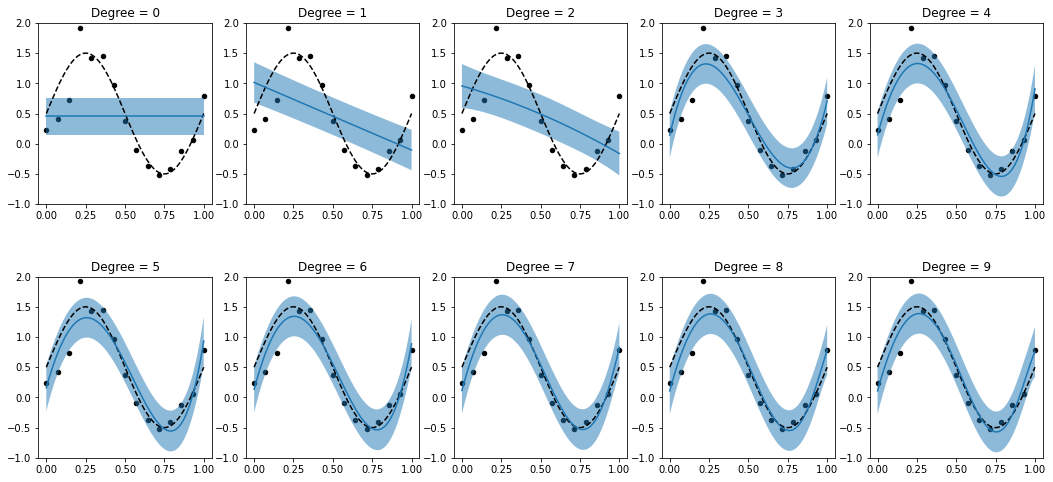
\includegraphics[width=3.4in]{figs/fig1.png}
\end{center}
\caption{}
\label{fig:1}
\end{figure}

From the above figure , we can observe that polynomial models of higher degree do not overfit to the data.

The following block plots the log of marginal likelihood vs Polynomial degree
\begin{lstlisting}
mlls = []

for d in degrees:
    mll = log_marginal_likelihood(Phi[:,:d+1], t, alpha=alpha, beta=beta)
    mlls.append(mll)

degree_max = np.argmax(mlls)
    
plt.plot(degrees, mlls)
plt.axvline(x=degree_max, ls='--', c='k', lw=1)
plt.xticks(range(0, 10))
plt.xlabel('Polynomial degree')
plt.ylabel('Log marginal likelihood');
\end{lstlisting}

\begin{figure}[!h]
\begin{center}
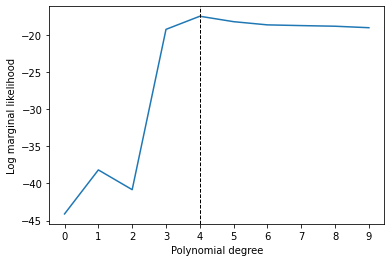
\includegraphics[width=3.4in]{figs/fig2.png}
\end{center}
\caption{}
\label{fig:2}
\end{figure}

Python code:
\begin{lstlisting}
https://github.com/Hrithikraj2/EE4015_IDP/blob/main/Assignment_7/Assignment_7.ipynb
\end{lstlisting}
\end{document}
